\documentclass[crop,tikz]{standalone}
\usetikzlibrary{backgrounds}
\colorlet{blue}{cyan}
\tikzset{
  inverted/.style = {
    color=white,
    background rectangle/.style={fill},
    show background rectangle
  }
}

\usepackage{pgfplots}
\usepackage{siunitx}
\tikzset{>=latex}

\pgfplotsset{
  inverted/.style = {
    every axis legend/.append style={
      draw=white,
      fill=black,
      text=white
    }
  },
  every non boxed x axis/.append style={
    axis line style={-latex}
  },
  every non boxed y axis/.append style={
    axis line style={-latex}
  }
}

\begin{document}
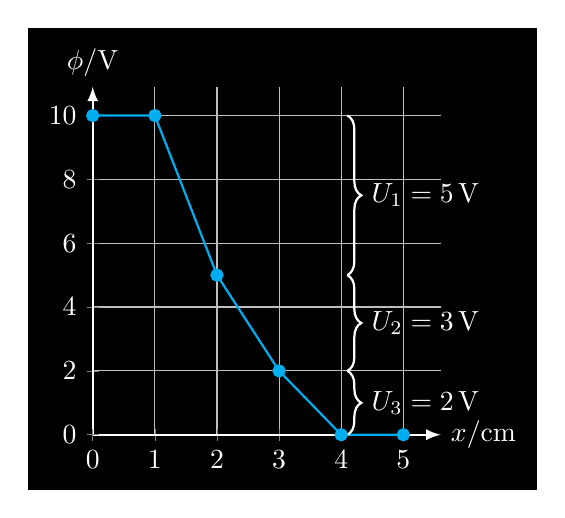
\begin{tikzpicture}[inverted,inverted]
  \begin{axis}[inverted,
    thick,
    width={6cm},
    height={6cm},
    axis y line=middle,
    axis x line=middle,
    xlabel={$x/\si{\cm}$},
    ylabel={$\phi/\si{\V}$},
    x label style={right},
    y label style={above},
    xtick distance=1,
    ytick distance=2,
    extra x ticks={0},
    extra x tick style={grid=none},
    extra y ticks={0},
    extra y tick style={grid=none},
    xmin=0, xmax=5.6,
    ymin=0, ymax=10.9,
    clip=false,
    grid
    ]
    \addplot[blue, thick, mark=*] plot coordinates {
      (0, 10)
      (1, 10)
      (2,  5)
      (3,  2)
      (4,  0)
      (5,  0)
    };
    \draw[decorate, decoration = {brace, amplitude=5pt}] (axis cs:4.1,10) -- ++(axis cs:0,-5) node[right,xshift=0.5em,midway] {$U_1=\SI{5}{\V}$};
    \draw[decorate, decoration = {brace, amplitude=5pt}] (axis cs:4.1,5)  -- ++(axis cs:0,-3) node[right,xshift=0.5em,midway] {$U_2=\SI{3}{\V}$};
    \draw[decorate, decoration = {brace, amplitude=5pt}] (axis cs:4.1,2)  -- ++(axis cs:0,-2) node[right,xshift=0.5em,midway] {$U_3=\SI{2}{\V}$};
  \end{axis}
\end{tikzpicture}
\end{document}
